\documentclass[a4paper,nofonts,raggedright,notitlepage]{tufte-handout}

% \usepackage[utf8]{inputenc}
% \usepackage[T1]{fontenc}

\usepackage{ifxetex}
\usepackage{fontspec}
\setmainfont[Ligatures=TeX,Numbers=OldStyle]{Cardo}
\setsansfont[Scale=0.94]{Cabin}
\setmonofont[Scale=0.94]{Consolas}
\usepackage{fontawesome}

\newcommand\sectionnote[1]{\marginnote{\color{RubineRed}#1}}

\ifxetex
  \newcommand{\textls}[2][5]{%
    \begingroup\addfontfeatures{LetterSpace=#1}#2\endgroup
  }
  \renewcommand{\allcapsspacing}[1]{\textls[15]{#1}}
  \renewcommand{\smallcapsspacing}[1]{\textls[10]{#1}}
  \renewcommand{\allcaps}[1]{\textls[15]{\MakeTextUppercase{#1}}}
  \renewcommand{\smallcaps}[1]{\smallcapsspacing{\scshape\MakeTextLowercase{#1}}}
  \renewcommand{\textsc}[1]{\smallcapsspacing{\textsmallcaps{#1}}}
\fi

%% Font settings suggested by fbb documentation.
% \usepackage{textcomp} % to get the right copyright, etc.
% \usepackage[lining,tabular]{fbb} % so math uses tabular lining figures
% \usepackage[scaled=.94,type1]{cabin} % sans serif in style of Gill Sans
% \usepackage[varqu,varl]{zi4}% inconsolata typewriter
% \useosf % change normal text to use proportional oldstyle figures
%\usetosf would provide tabular oldstyle figures in text

\setsidenotefont{\sffamily\footnotesize}
\setmarginnotefont{\sffamily\footnotesize}
\setcaptionfont{\sffamily\itshape\footnotesize}

\usepackage[os=win]{menukeys}
\usepackage{graphicx}

\setcounter{secnumdepth}{3}
\usepackage{enumitem}
\setlist{noitemsep}

\usepackage{minted}

\title[Guide on Using upnmthesis]{Guide on Using \texttt{upnmthesis} for Writing Universiti Pertahanan Nasional Malaysia Theses with \LaTeX}
\date{version 1.0, October 20, 2015}
\author{Lian Tze Lim, Ph.D. (liantze\string@gmail.com)}

\begin{document}

\maketitle

\begin{abstract}
\texttt{upnmthesis} is a \LaTeX\ class \marginnote{The latest version of this template can be downloaded from \url{http://liantze.penguinattack/latextypesetting.html\#upnmthesis}.} for authoring theses that fulfil formatting specifications required by Universiti Pertahanan Nasional Malaysia (\textsc{upnm}). This class and template was commissioned by the university's Centre of Graduate Studies in October, 2015, for both undergraduate and postgraduate theses.

A sample \texttt{sample-thesis.tex}, as well as relevant sample chapters, are included in the package,\marginnote{\texttt{upnmthesis} is available as a template on Overleaf.} which I recommend you modify for your own thesis write-up. (You can rename it, but I'll stick with the file name `\texttt{sample-thesis.tex}' throughout this guide.)
\end{abstract}


\medskip

\section{Compiling the Template the Easy Way}\sectionnote{\faCloud{} In the cloud!}
You may want to consider writing your thesis in the cloud, so that you won't have to maintain your own local \LaTeX{} installation or setting up the processing tools.

There are now a number of \LaTeX{} cloud editing platforms, e.g.~Overleaf, \marginnote{Disclosure: I'm the Community \TeX{}pert at Overleaf.} ShareLaTeX, Authorea, etc. The \textsc{upnm} thesis template is available on Overleaf.


\section{Configuring TeXworks to Compile \texttt{upnmthesis}}\label{sec:texworks}\sectionnote{\faGears{} Configs for TeXworks. Other editors should have something similar.}
Assuming TeXworks is your \LaTeX\ editor of choice, you will probably want to configure it so that you can process your glossary and list of own publications from within TeXworks.
You should work through this section to ensure that you are able to compile the sample thesis successfully.

(You can always, of course, opt to run the relevant commands from the command line prompt, or adapt these configurations for other editors and operating systems.)

%This section will also mention a few things to note when compiling and printing your thesis.

\subsection{Tool Configuration for Generating the List of Acronyms}\label{sec:texworks:makeglossaries}
Access the TeXworks menu \menu{Edit > Preferences > Typesetting}. Add a new processing tool called `List of Acronyms'. Configure it as shown in Figure~\ref{fig:texworks:acronyms} (p.\pageref{fig:texworks:acronyms}).

\begin{figure}
\centering
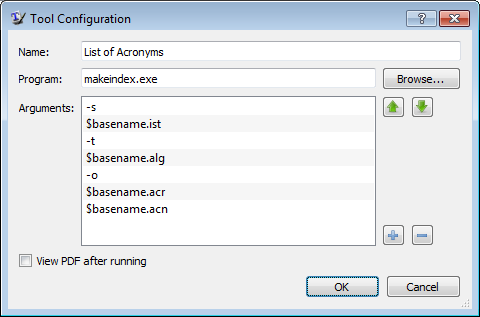
\includegraphics[width=.8\textwidth]{texworks-acronyms}
\caption{Setting up the `List of Acronyms' processing tool in TeXworks}
\label{fig:texworks:acronyms}
\end{figure}

On Linux and Mac systems, this is equivalent to the command line

\begin{fullwidth}
\begin{minted}{bash}
$  makeindex -s <basename>.ist -t <basename>.alg -o <basename>.acr <basename>.acn
\end{minted}
\end{fullwidth}

\marginnote[0.5em]{where \texttt{<basename>} is the name of your main file (i.e.~\texttt{sample-thesis}).}


\subsection{Tool Configuration for Generating the List of Publications}
Add another processing tool called ``Publication List''. Configure it as shown in Figure~\ref{fig:texworks:publist} (p.~\ref{fig:texworks:publist}).
On Linux and Mac systems, this is equivalent to the command line

\begin{minted}{bash}
$  bibtex own
\end{minted}

\begin{figure}
\centering
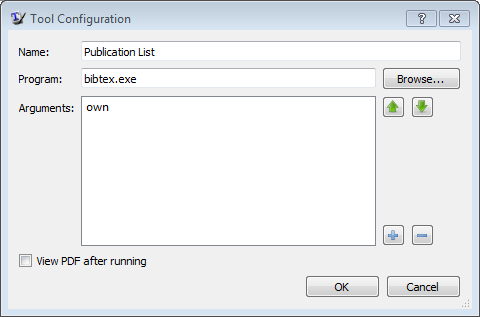
\includegraphics[width=.8\textwidth]{texworks-publist}
\caption{Setting up the `Publication List' processing tool in TeXworks}
\label{fig:texworks:publist}
\end{figure}



\subsection{Compiling \texttt{thesis.tex}}\sectionnote{\faCode{} Compilation steps}
When using TeXworks, the processing tools should be run on \texttt{thesis.tex} in the following sequence:
\begin{enumerate}
\item pdfLaTeX + BibTeX + Makeindex
\item List of Acronyms
\item Publication List
\item pdfLaTeX + BibTeX + Makeindex
\end{enumerate}

You will need to run `List of Acronyms' again if you add and use a new acronym. Similarly, run `Publication List' again if you add a new self publication. Don't forget to run `pdfLaTeX + BibTeX + Makeindex' after that!

\subsection{Why is there a blank page before the title page and at the end?!}\sectionnote{\faQuestion\faExclamation{} What, blank pages?!}
The thesis preparation guidelines say there needs to be a blank page between the cover and the title page, and another at the very end, so \textsf{umalayathesis} forces one just in case you forgot to insert one. \faSmileO

\subsection{Printing from Acrobat Reader}\sectionnote{\faPrint{} Make sure the print out isn't shrunk!}
Remember to set the \textbf{paper size} to \textbf{A4} and \textbf{page scaling} to \textbf{None} in the \textsf{Print} dialog, otherwise the margins would be incorrect.


\end{document}